\chapter{Implementation}
\label{chapter:Implementation}

In this chapter, we discuss implementation details of our approach discussed in 
\ref{chapter:Methods}. The first section discusses the creation of a annotated dataset 
for train sepparatly the part based detection algorithm and the template based, while 
in the second section, we describe....the implementation 
of the c++ algorithm \todo{....}
 
 \section{Dataset - Part based model}
 In this section, We discuss the details involve in the creation of the dataset for
 train the algorithm define in \ref{chapter:Methods}, during the project we acquire
 a big amount of data, considering different in daylight light, water properties and
 with different fish types, but for this work, and due that the data preparation is 
 handwork intensely, we process a specific set of data, in which all the experiment
 were realized, to achieve this goal, a small C++ application was developed for this.
 and as discuss, in \ref{chapter:Methods} the fish is model using the concept of stickmen,
 and is use two fish model with 3 and 7 parts, based on this data, then the model can be 
 extrapolate to 5, 9, 11 part model.


\begin{equation}
\hat{point}_{m'xn} =\mathtt{A}_{m'xm} \cdot point_{mxn}
\end{equation}

where
 \begin{equation}
 \label{eq:extrapole}
\mathtt{A} =
\begin{bmatrix}
a_{11}  & a_{12}  & 0 & \cdots & \cdots & \cdots & \cdots & 0 \\
a_{21}  & a_{22}  & a_{23}  & \ddots & && & \vdots \\
0 & a_{32}  & a_{33} & a_{34}  & \ddots & &  & \vdots \\
\vdots & \ddots & \ddots & \ddots & \ddots & \ddots &  & \vdots \\
\vdots & & \ddots & \ddots & \ddots & \ddots & \ddots& \vdots\\
\vdots  &  & & \ddots & a_{(m'-2)(m-3)}  & a_{(m'-2)(m-2)}  &  a_{(m'-2)(m-1)}  & 0\\
\vdots  &  & & & \ddots & a_{(m'-1)(m-2)}  & a_{(m'-1)(m_1)}  &  a_{(m'-1)m}\\
0 & \cdots &  \cdots & \cdots & \cdots & 0 & a_{m'(m-1)} & a_{m'm}  \\
\end{bmatrix}
 \end{equation}


\begin{figure}
\begin{adjustwidth}{-1in}{-1in} 
\label{fig:anotated1}
\centering     %%% not \center
\subfigure[]{\label{fig:a}\includegraphics[width=70mm]{anotated/3/data_st11_led0_0021}}
\subfigure[]{\label{fig:a}\includegraphics[width=70mm]{anotated/3/data_st11_led0_0023}}
\subfigure[]{\label{fig:a}\includegraphics[width=70mm]{anotated/3/data_st11_led0_0025}}
\subfigure[]{\label{fig:a}\includegraphics[width=70mm]{anotated/3/data_st11_led0_0027}}
\caption{This illustrates the annotated fish in a 3 Part model}
\end{adjustwidth}
\end{figure}

\begin{figure}
\begin{adjustwidth}{-1in}{-1in} 
\label{fig:anotated1}
\centering     %%% not \center
\subfigure[]{\label{fig:a}\includegraphics[width=70mm]{anotated/5/data_st11_led0_0021}}
\subfigure[]{\label{fig:a}\includegraphics[width=70mm]{anotated/5/data_st11_led0_0023}}
\subfigure[]{\label{fig:a}\includegraphics[width=70mm]{anotated/5/data_st11_led0_0025}}
\subfigure[]{\label{fig:a}\includegraphics[width=70mm]{anotated/5/data_st11_led0_0027}}
\caption{This illustrates the annotated fish in a 7 Part model}
\end{adjustwidth}
\end{figure}

now as a example, to extrapolate from a 3 parts model to a 5 parts model, the matrix
should look like this:


\begin{equation}
\hat{point}_{9'x2} =\mathtt{A}_{5'x3} \cdot point_{3x2}
\end{equation}

where
 \begin{equation}
 \label{eq:extrapole}
\mathtt{A} =
\begin{bmatrix}
1  & 0 & 0 & 0 & 0 & 0 & 0 \\
\frac{1}{2} & \frac{1}{2}  & 0 & 0 & 0 & 0 & 0 \\
0 & 1  & 0 & 0 & 0 & 0 & 0  \\
0 & \frac{1}{2} & \frac{1}{2} & 0 & 0 & 0 & 0 \\
0  & 0 & 1 & 0 & 0 & 0 & 0  \\
0  & 0 & 0 & 1 & 0 & 0 & 0  \\
0  & 0 & 0 & 0 & 1 & 0 & 0 \\
0  & 0 & 0 & 0 & 0 & 1 & 0 \\
0  & 0 & 0 & 0 & 0 & 0 & 1  \\
\end{bmatrix}
 \end{equation}

and each $\frac{1}{2}$ represent the middle point between the two original annotated
points.

\begin{figure}
\begin{adjustwidth}{-1in}{-1in} 
\label{fig:anotated1}
\centering     %%% not \center
\subfigure[]{\label{fig:a}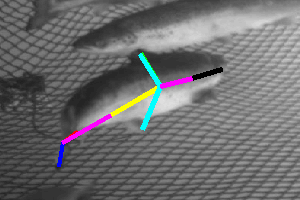
\includegraphics[width=70mm]{anotated/9_extra/extra_9_01}}
\subfigure[]{\label{fig:a}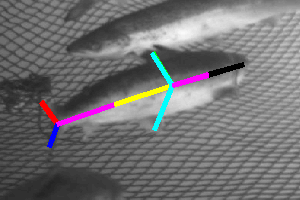
\includegraphics[width=70mm]{anotated/9_extra/extra_9_02}}
\caption{This illustrates the annotated fish in a 9 Part model, where is clearly visible
the new points define in the middle point of the existent parts.}
\end{adjustwidth}
\end{figure}

 \section{Dataset - Templated based model based model}
 In this section, We discuss the details involve in the creation of the dataset for
 train the algorithm define in \ref{chapter:Methods}, as said before for the template matching algorithm, we propose a different way to generate the proper templates, we have template for the Head and Tail, and we train to different detector, in the fig:\todo{ref}

\begin{figure}
\begin{adjustwidth}{-1in}{-1in} 
\label{fig:head_1}
\centering     %%% not \center
\subfigure[]{\label{fig:a}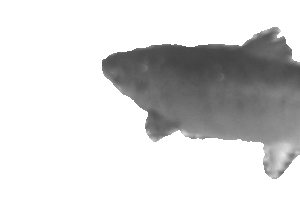
\includegraphics[width=40mm]{anotated/linemod/head/data_st11_led0_0219-4}}
\subfigure[]{\label{fig:a}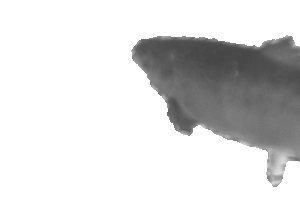
\includegraphics[width=40mm]{anotated/linemod/head/data_st11_led0_0221-4}}
\subfigure[]{\label{fig:a}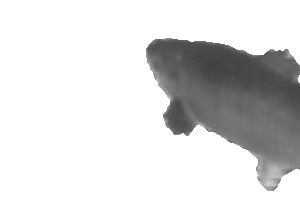
\includegraphics[width=40mm]{anotated/linemod/head/data_st11_led0_0223-4}}
\subfigure[]{\label{fig:a}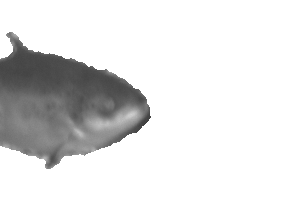
\includegraphics[width=40mm]{anotated/linemod/head/data_st11_led0_0227-4}}
\subfigure[]{\label{fig:a}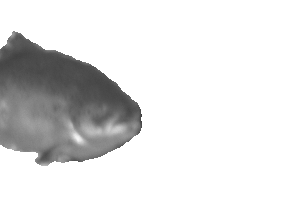
\includegraphics[width=40mm]{anotated/linemod/head/data_st11_led0_0229-4}}
\subfigure[]{\label{fig:a}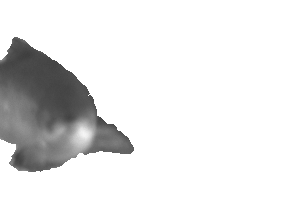
\includegraphics[width=40mm]{anotated/linemod/head/data_st11_led0_0231-4}}
\subfigure[]{\label{fig:a}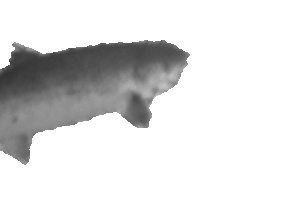
\includegraphics[width=40mm]{anotated/linemod/head/data_st11_led0_0233-4}}
\subfigure[]{\label{fig:a}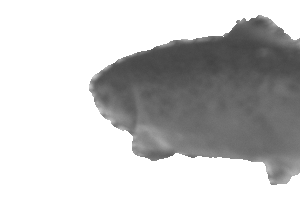
\includegraphics[width=40mm]{anotated/linemod/head/data_st11_led0_0235-4}}
\caption{This illustrates the annotated fish in a 7 Part model}
\end{adjustwidth}
\end{figure}

\begin{figure}
\begin{adjustwidth}{-1in}{-1in} 
\label{fig:head_2}
\centering     %%% not \center
\subfigure[]{\label{fig:a}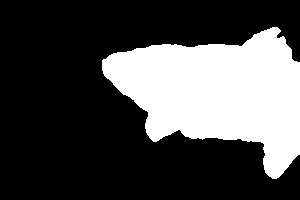
\includegraphics[width=40mm]{anotated/linemod/head/data_st11_led0_0219-3}}
\subfigure[]{\label{fig:a}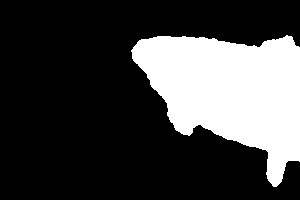
\includegraphics[width=40mm]{anotated/linemod/head/data_st11_led0_0221-3}}
\subfigure[]{\label{fig:a}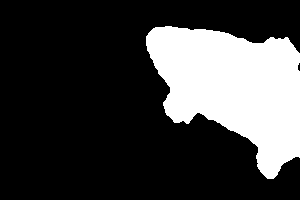
\includegraphics[width=40mm]{anotated/linemod/head/data_st11_led0_0223-3}}
\subfigure[]{\label{fig:a}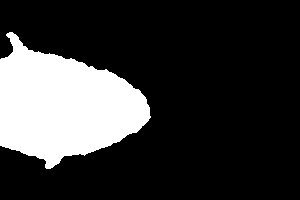
\includegraphics[width=40mm]{anotated/linemod/head/data_st11_led0_0227-3}}
\subfigure[]{\label{fig:a}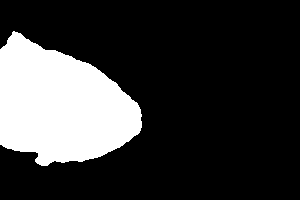
\includegraphics[width=40mm]{anotated/linemod/head/data_st11_led0_0229-3}}
\subfigure[]{\label{fig:a}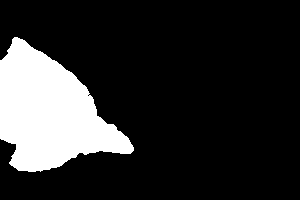
\includegraphics[width=40mm]{anotated/linemod/head/data_st11_led0_0231-3}}
\subfigure[]{\label{fig:a}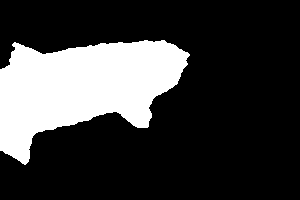
\includegraphics[width=40mm]{anotated/linemod/head/data_st11_led0_0233-3}}
\subfigure[]{\label{fig:a}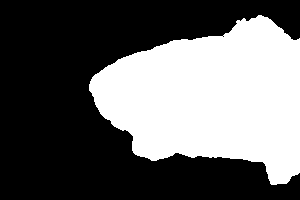
\includegraphics[width=40mm]{anotated/linemod/head/data_st11_led0_0235-3}}
\caption{This illustrates the annotated fish in a 7 Part model}
\end{adjustwidth}
\end{figure}

\begin{figure}
\begin{adjustwidth}{-1in}{-1in} 
\label{fig:tail_1}
\centering     %%% not \center
\subfigure[]{\label{fig:a}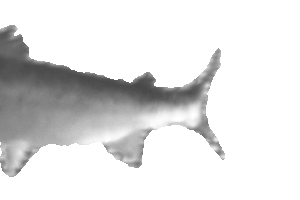
\includegraphics[width=40mm]{anotated/linemod/tail/data_st11_led0_0219-6}}
\subfigure[]{\label{fig:a}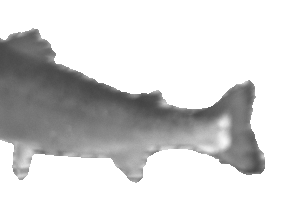
\includegraphics[width=40mm]{anotated/linemod/tail/data_st11_led0_0221-6}}
\subfigure[]{\label{fig:a}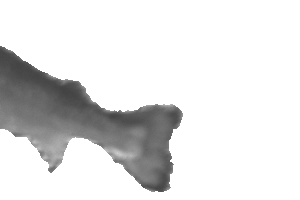
\includegraphics[width=40mm]{anotated/linemod/tail/data_st11_led0_0223-6}}
\subfigure[]{\label{fig:a}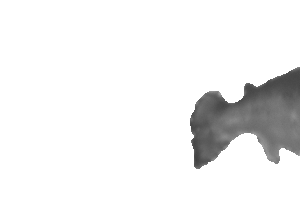
\includegraphics[width=40mm]{anotated/linemod/tail/data_st11_led0_0227-6}}
\subfigure[]{\label{fig:a}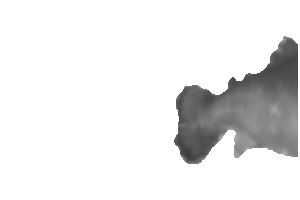
\includegraphics[width=40mm]{anotated/linemod/tail/data_st11_led0_0229-6}}
\subfigure[]{\label{fig:a}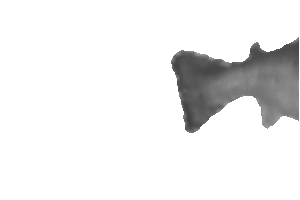
\includegraphics[width=40mm]{anotated/linemod/tail/data_st11_led0_0231-6}}
\subfigure[]{\label{fig:a}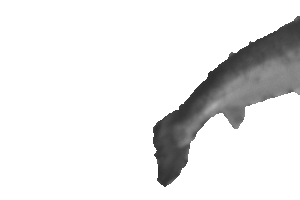
\includegraphics[width=40mm]{anotated/linemod/tail/data_st11_led0_0233-6}}
\subfigure[]{\label{fig:a}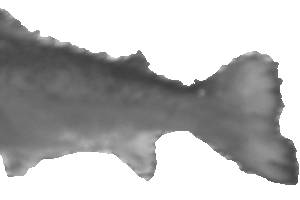
\includegraphics[width=40mm]{anotated/linemod/tail/data_st11_led0_0235-6}}
\caption{This illustrates the annotated fish in a 7 Part model}
\end{adjustwidth}
\end{figure}

\begin{figure}
\begin{adjustwidth}{-1in}{-1in} 
\label{fig:tail_2}
\centering     %%% not \center
\subfigure[]{\label{fig:a}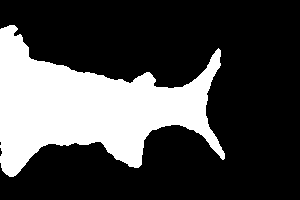
\includegraphics[width=40mm]{anotated/linemod/tail/data_st11_led0_0219-5}}
\subfigure[]{\label{fig:a}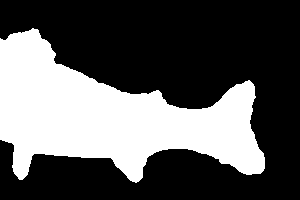
\includegraphics[width=40mm]{anotated/linemod/tail/data_st11_led0_0221-5}}
\subfigure[]{\label{fig:a}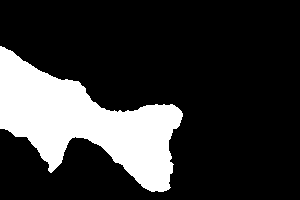
\includegraphics[width=40mm]{anotated/linemod/tail/data_st11_led0_0223-5}}
\subfigure[]{\label{fig:a}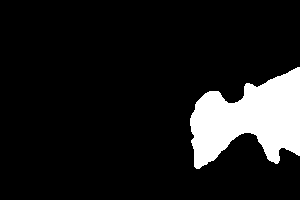
\includegraphics[width=40mm]{anotated/linemod/tail/data_st11_led0_0227-5}}
\subfigure[]{\label{fig:a}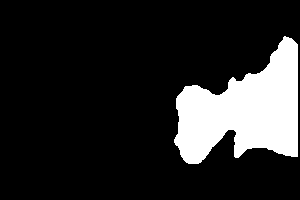
\includegraphics[width=40mm]{anotated/linemod/tail/data_st11_led0_0229-5}}
\subfigure[]{\label{fig:a}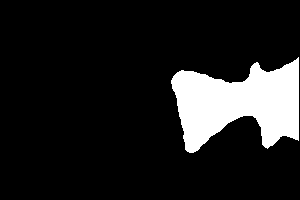
\includegraphics[width=40mm]{anotated/linemod/tail/data_st11_led0_0231-5}}
\subfigure[]{\label{fig:a}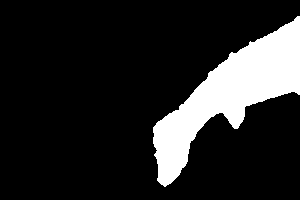
\includegraphics[width=40mm]{anotated/linemod/tail/data_st11_led0_0233-5}}
\subfigure[]{\label{fig:a}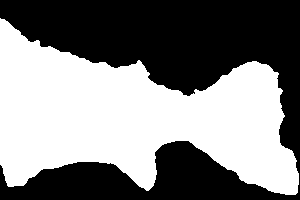
\includegraphics[width=40mm]{anotated/linemod/tail/data_st11_led0_0235-5}}
\caption{This illustrates the annotated fish in a 7 Part model}
\end{adjustwidth}
\end{figure}

\section{Linemod}
There is no need for a latex introduction since there is plenty of literature out there.


% \section{Next Section}
% There is no need for a latex introduction since there is plenty of literature out there.
